\documentclass{beamer}

\usepackage{minted}

\usetheme{CambridgeUS}
\setbeamercolor{enumerate item}{fg=black}

\title[Stratégies dans LoL] %optional
{Analyse de stratégies générales dans League of Legends Arbres de décision et sous-graphes fréquents}
\author{Julien BOURDET}
\institute{37797}
\date[] %optional
{TIPE 2024}

\AtBeginSection[]
{
  \begin{frame}
    \frametitle{Sommaire}
    \tableofcontents[currentsection]
  \end{frame}
}

\begin{document}

\frame{\titlepage}

\section{Concept}

\begin{frame}
    \frametitle{League of Legends\cite{league}}
    \begin{figure}[h]
        \centering
        \includegraphics[width=0.80\linewidth]{image.png}
        \caption{Capture d'écran du jeu}
    \end{figure}
\end{frame}

\begin{frame}
    \frametitle{Pourquoi ?}
    \begin{columns}
        \column{0.4\textwidth}
        \begin{figure}
            \centering
            \includegraphics[width=0.6\linewidth]{esport.png}
            \caption{Photo prise en Corée}
        \end{figure}
        \column{0.5\textwidth}
        \begin{figure}
            \centering
            \includegraphics[width=1\linewidth]{esport2.png}
            \caption{Stade pour une finale}
        \end{figure}
    \end{columns}
\end{frame}

\begin{frame}
    \frametitle{Objectif}
    \begin{enumerate}
        \item[$\bullet$] Étude de 2014 sur DOTA 2\cite{yang}. \newline \newline
        \item[$\bullet$] Application à LoL.
    \end{enumerate}
    \begin{figure}
        \centering
        \includegraphics[width=0.2\linewidth]{python.png}
        \caption{Python}
    \end{figure}
\end{frame}

\section{Méthode}

\begin{frame}
    \frametitle{Construire les graphes}
    \begin{block}{Définition}
        On dit que deux joueurs ont interagit si ils se sont attaqués. 
    \end{block}
    \begin{block}{Définition}
        Soit $G_{i}^{j} = (S, A)$ le graphe orienté d'interactions de la partie $j$, dans le laps de temps $i$. \newline\newline
        Les sommets de $S$ sont tous les joueurs de la partie $j$. On ajoute aussi un sommet pour la mort qu'on note $d$. \newline\newline
        Si pendant le laps de temps $i$, le joueur $s \in S$ a interagit avec le joueur $t \in S$, alors $(s, t) \in A$, de plus si le joueur $s$ est mort alors $(s, d) \in A$.
    \end{block}
\end{frame}

\begin{frame}
    \frametitle{Construire les graphes}
    \begin{columns}
        \column{0.5\textwidth}
        \begin{figure}
            \centering
            \includegraphics[width=0.9\linewidth]{graph_1.png}
            \caption{Graphe 1}
        \end{figure}
        \column{0.5\textwidth}
        \begin{figure}
            \centering
            \includegraphics[width=0.9\linewidth]{graph_2.png}
            \caption{Graphe 2}
        \end{figure}        
        \end{columns}
\end{frame}

\begin{frame}
    \frametitle{Caractéristiques de graphes}\small
    Pour chaque graphe $G_{i}^{j}$ on récupère des caractéristiques. \newline \newline
    On appelle caractéristique, toute fonction sur le graphe, ou un de ses sommets, qui renvoie un réel. Par exemple, le degré entrant et sortant d'un sommet, la centralité de proximité ou la centralité d'intermédiarité du graphe. \newline
    \begin{block}{Définition}
        Soit $f$, qui prend un graphe $G_{i}^{j}$ et renvoit ses caractéristiques.
    \end{block}
    \begin{block}{Définition}
        Soit $g$, qui prend un graphe $G_{i}^{j}$ et renvoit si la partie $j$ à été gagnée.
    \end{block}
\end{frame}

\begin{frame}
    \frametitle{Algorithme C4.5}
    On utilise alors l'algorithme C4.5\cite{c4.5}, pour créer un arbre de décision. \newline \newline
    \begin{figure}
        \centering
        \includegraphics[width=1\linewidth]{tree.png}
        \caption{Arbre de décision}
    \end{figure}
\end{frame}

\begin{frame}
    \frametitle{Règles de combat}
    \footnotesize
    On crée alors, à partir de cet arbre de décision des règles de combat. Une règle est le tracé d'une feuille vers le sommet de l'arbre. \newline \newline
    Ici, une des règles serait: \newline \newline
    "SI degré sortant du role 5 dans l'équipe 1 dans le laps de temps 11 $<$ 0.1452 ET degré entrant du role 1 dans l'équipe 1 dans le laps de temps 8 $\ge$ 3.0561 ALORS l'équipe 2 gagne”.
    \begin{figure}
        \centering
        \includegraphics[width=0.9\linewidth]{written_tree.png}
        \caption{Arbre de décision, règle en rouge}
    \end{figure}
\end{frame}

\begin{frame}
    \frametitle{Minage de sous-graphes fréquents\cite{fsm}}
    \begin{block}{Définition}
        Soit $r(j) = \left\{
        \begin{array}{ll}
            vrai & \mbox{si la partie } j \mbox{ respecte cette règle}\\
            faux & \mbox{sinon.}
        \end{array}
        \right.$
    \end{block}
    \begin{block}{Définition}
        $\forall i$, et pour $s \in [0,1]$ le support \\
        On note les $n$ sous-graphes fréquents des graphes $G_{i}^{j}$, tels que $r(j) = vrai$ : \\
        $\forall k \in [\![1,n]\!]$, $F^{i}_{k}$ est un sous-graphe d'au moins un des $G_{i}^{j}$, et apparait dans plus de $s \times \lvert G_{i}^{j} \rvert$ graphes.
    \end{block}
\end{frame}

\section{Importer les données}

\begin{frame}
    \frametitle{Récupérer des parties}
    \begin{columns}
        \column{0.5\textwidth}
        \begin{enumerate}
            \item[$\bullet$]\footnotesize En utilisant le site League Of Graphs\cite{leaguegraphs} on récupère des identifiants de parties.
            \item[$\bullet$] Sous la forme $/region/id$. \newline
            ie. $/kr/6890257502$
            \item[$\bullet$] Elles ne sont pas aléatoires.
        \end{enumerate}
        \column{0.5\textwidth}
        \begin{figure}
            \centering
            \includegraphics[width=1\linewidth]{leagueofgraphs.png}
            \caption{https://www.leagueofgraphs.com}
        \end{figure}
    \end{columns}
\end{frame}

\begin{frame}
    \frametitle{Récupérer des parties}
    \begin{figure}
        \centering
        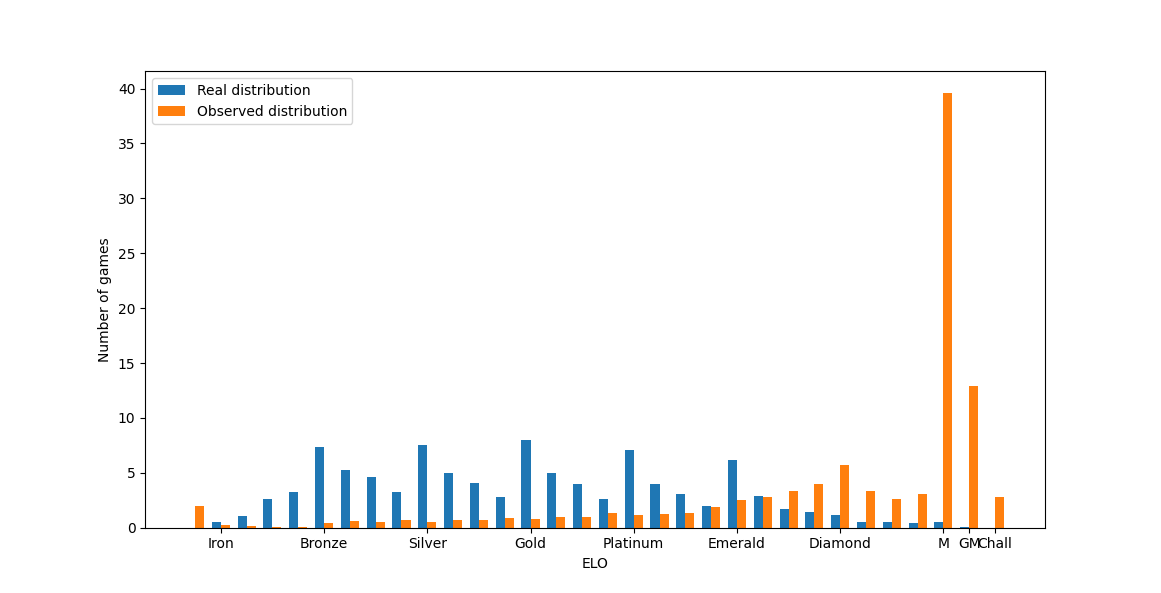
\includegraphics[width=1\linewidth]{elo_distribution.png}
        \caption{Elo distribution}
    \end{figure}
\end{frame}

\begin{frame}
    \frametitle{Récupérer des parties}
    \begin{figure}
        \centering
        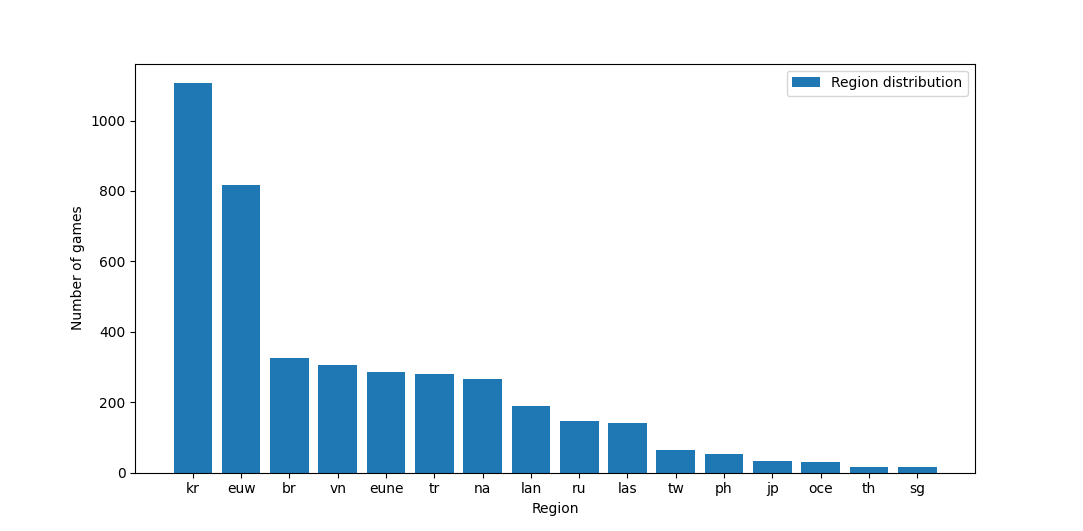
\includegraphics[width=1\linewidth]{region_distribution.png}
        \caption{Region distribution}
    \end{figure}
\end{frame}

\begin{frame}
    \frametitle{Récupérer des parties}
    \begin{enumerate}
        \item[$\bullet$] L'API de Riot Games ne permet pas de récupérer les informations nécessaires.
        \item[$\bullet$] Contact d'un dévloppeur de Riot Games.
        \item[$\bullet$] LiveEvents API\cite{liveevents}. \newline
    \end{enumerate}
\end{frame}

\begin{frame}[fragile]
    \frametitle{LiveEvents API}
    \begin{enumerate}
        \item[$\bullet$] Quand on regarde un Replay, le jeu envoit un flux de donnée sur un port (34243) contenant tout les évènements se déroulant dans le Replay. \\
        On utilise ces évènements pour construire les graphes $G_{i}^{j}$.
    \end{enumerate}
    \begin{figure}
        \centering
        \tiny
            \begin{verbatim}
                                    {
                                        "eventname": "OnGameStart",
                                        "timestamp": "1704622679.621711"
                                    },
                                    {
                                        "eventname": "OnDamageGiven",
                                        "other": "daleste",
                                        "otherID": "6",
                                        "otherTeam": "Chaos",
                                        "source": "Will",
                                        "sourceID": "4",
                                        "sourceTeam": "Order",
                                        "timestamp": "1704622699.994257"
                                    },
        \end{verbatim}
        \caption{Exemple d'évènements}
    \end{figure}
\end{frame}

\section{Algorithme génétique}

\begin{frame}
    \frametitle{Problématique}
    \begin{enumerate}
        \item[$\bullet$] Il y en a $30 \times 11 \times 5 = 1650$ caractérstiques.
        \item[$\bullet$] Quand on créé l'arbre de décision, on ne peut pas utiliser toutes les caractéristiques possibles. Dans ce cas, l'arbre créé couvrerait toutes les données. Il y aurait suraprentissage\cite{overfitting}.
        \item[$\bullet$] Il faut donc trouver un minimun de caractéristiques qui produisent l'arbre le plus précis possible.
    \end{enumerate}
\end{frame}

\begin{frame}
    \frametitle{Algorithme génétique}
    On utilise alors un algorithme génétique\cite{gary} pour trouver ces caractéristiques.
\end{frame}

\section{References}

\begin{frame}{References}
    \scriptsize
    \begin{thebibliography}{9}
        \setbeamertemplate{bibliography item}[text]
        \setbeamercolor{bibliography item}{parent=palette primary}
        \setbeamercolor*{bibliography entry author}{fg=black}
        \bibitem{league}
            Riot Games.
            “League of Legends”, 2009.
            \emph{https://www.riotgames.com/}
        \bibitem{yang}
            Yang, Pu, Brent E. Harrison, and David L. Roberts.
            "Identifying patterns in combat that are predictive of success in MOBA games."
            \emph{FDG. 2014.}
        \bibitem{leaguegraphs}
            WARGRAPHS.
            \emph{https://www.leagueofgraphs.com/}
        \bibitem{overfitting}
            Max B. (2007).
            Avoiding Overfitting of Decision Trees.
            In: \emph{Principles of Data Mining.}
            Springer, London
        \bibitem{gary}
            Gary S., Bing C., Annie S. W., and Kien A. H.. (2005).
            Decision tree classifier for network intrusion detection with GA-based feature selection.
            In \emph{Proceedings of the 43r annual Southeast regional conference}
            - Volume 2 (ACM-SE 43), Vol. 2. Association for Computing Machinery, New York, NY, USA, 136–141.
        \bibitem{c4.5}
            Quinlan, J. R.
            “C4.5: Programs for Machine Learning”.
            Morgan Kaufmann Publishers, 1993.
        \bibitem{fsm}
            Chi, Y., Muntz, R. R., Nijssen, S., \& Kok, J. N. (2005).
            Frequent subtree mining–and overview.
            \emph{Fundamenta Informaticae},
            66(1-2), 161-198.
        \bibitem{liveevents}
            \emph{https://github.com/SkinSpotlights/LiveEventsDocumentation}
    \end{thebibliography}
\end{frame}

\section{Annexes}

%classes/c45.py

\begin{frame}[fragile]
    \frametitle{Code}
    \scriptsize
    classes/c45.py \newline
    \fontsize{3pt}{5pt}\selectfont
    \begin{minted}{python}
import math
import random


class Node:
    """
    A class to represent a node in a decision tree.
    """
    def __init__(self, is_leaf: bool, label: str, threshold: float) -> None:
        self.label = label
        self.threshold = threshold
        self.is_leaf = is_leaf
        self.children = []

        
class C45:
    """
    A class to represent a C4.5 decision tree.
    """
    def __init__(self, data, classes: list[str], features: list[str]) -> None:
        self.data = data
        self.classes = classes
        self.features = features

        self.tree = None

    def get_majority_class(self, data) -> str:
        """
        Returns the class that appears the most in the data.
        """

        return max(set([e["class"] for e in data]), key=[e["class"] for e in data].count)
    
    def split_attribute(self, data, features: list[str]):
        """
        Splits the data on the best attribute and threshold.
        """

        splitted_data = []
        best_feature: str
        best_threshold: float
    \end{minted}
\end{frame}

\begin{frame}[fragile]
    \frametitle{Code}
    \fontsize{3pt}{5pt}\selectfont
    \begin{minted}{python}
        max_gain = -1
        
        for feature in features:
            sorted_data = sorted(data, key=lambda x: x[feature])
            for i in range(len(sorted_data) - 1):
                threshold = (sorted_data[i][feature] + sorted_data[i + 1][feature]) / 2
                left = [e for e in sorted_data if e[feature] <= threshold]
                right = [e for e in sorted_data if e[feature] > threshold]
                gain = self.gain(data, left, right)
                if gain > max_gain:
                    max_gain = gain
                    splitted_data = [left, right]
                    best_feature = feature
                    best_threshold = threshold
                    
        return best_feature, best_threshold, [subset for subset in splitted_data if subset]
    
    def gain(self, parent, left, right):
        """
        Returns the information gain of the split.
        """

        return self.entropy(parent) - self.entropy(left) * len(left) / len(parent) - self.entropy(right) * len(right) / len(parent)
    
    def entropy(self, data):
        """
        Returns the entropy of the data.
        """

        if len(data) == 0:
            return 0
        classes = [e["class"] for e in data]
        return -1 * sum([classes.count(c) / len(data) * math.log(classes.count(c) / len(data), 2) for c in set(classes)])

    def generate_tree(self):
        """
        Generates the decision tree.
        """

        self.tree = self.__generate_tree_rec(self.data, self.features)

        
    def __generate_tree_rec(self, data, features):
    \end{minted}
\end{frame}

\begin{frame}[fragile]
    \frametitle{Code}
    \fontsize{3pt}{5pt}\selectfont
    \begin{minted}{python}
        """
        Recursively generates the decision tree.
        """
        
        # If all data is of the same class, return a leaf node with that class
        if len(set([e["class"] for e in data])) == 1:
            return Node(True, data[0]["class"], None)
        
        # If there are no more features to split on, return a leaf node with the majority class
        if len(features) == 0:
            return Node(True, self.get_majority_class(data), None)
        
        best_feature, best_threshold, splitted_data = self.split_attribute(data, features)
        remaining_features = features.copy()
        remaining_features.remove(best_feature)

        node = Node(False, best_feature, best_threshold)
        node.children = [self.__generate_tree_rec(subset, remaining_features) for subset in splitted_data]

        return node
    
    def print_node(self, node, depth=0):
        """
        Prints a node of the decision tree.
        """

        if node.is_leaf:
            return
        else:
            left = node.children[0]
            if left.is_leaf:
                print(' ' * depth + node.label + ' <= ' + str(node.threshold) + ' : ' + left.label)
            else:
                print(' ' * depth + node.label + ' <= ' + str(node.threshold) + ' : ')
                self.print_node(left, depth + 4)
            if len(node.children) == 2:
                right = node.children[1]

                if right.is_leaf:
                    print(' ' * depth + node.label + ' > ' + str(node.threshold) + ' : ' + right.label)
                else:
                    print(' ' * depth + node.label + ' > ' + str(node.threshold) + ' : ')
                    self.print_node(right, depth + 4)
    \end{minted}
\end{frame}

\begin{frame}[fragile]
    \frametitle{Code}
    \fontsize{3pt}{5pt}\selectfont
    \begin{minted}{python}
    def print_tree(self):
        """
        Prints the decision tree.
        """
        
        self.print_node(self.tree)

    def get_accuracy(self, split=None):
        """
        Returns the accuracy of the decision tree.
        """
                
        data = self.data.copy()
        if split:
            random.shuffle(data)
            data = data[:len(data) // split]

        return self.__get_accuracy_rec(self.tree, data) / len(data)
    
    def __get_accuracy_rec(self, node, data):
        """
        Recursively calculates the accuracy of the decision tree.
        """

        if node.is_leaf:
            return sum([1 for e in data if e["class"] == node.label])
        else:
            left_data = [e for e in data if e[node.label] <= node.threshold]
            if len (node.children) == 2:
                right_data = [e for e in data if e[node.label] > node.threshold]
                return self.__get_accuracy_rec(node.children[0], left_data) + self.__get_accuracy_rec(node.children[1], right_data)
            else:
                return self.__get_accuracy_rec(node.children[0], left_data)
        
    def predict(self, data):
        """
        Predicts the class of a data point.
        """

        return self.__predict_rec(self.tree, data)
    
    def __predict_rec(self, node, data):
    \end{minted}
\end{frame}

\begin{frame}[t, fragile]
    \frametitle{Code}
    \fontsize{3pt}{5pt}\selectfont
    \begin{minted}{python}
        """
        Recursively predicts the class of a data point.
        """

        if node.is_leaf:
            return node.label
        else:
            if data[node.label] <= node.threshold:
                return self.__predict_rec(node.children[0], data)
            else:
                return self.__predict_rec(node.children[1], data)
            
    def k_fold_cross_validation(self, k):
        """
        Performs k-fold cross validation.
        """
        
        save = self.data.copy()
        data = self.data.copy()
        data = [data[i::k] for i in range(k)]
        accuracies = []
        
        for i in range(k):
            test_data = data[i]
            train_data = []
            for j in range(k):
                if j != i:
                    train_data += data[j]
            
            self.data = train_data
            self.generate_tree()
            self.data = test_data
            accuracies.append(self.get_accuracy())
            
        self.data = save
        self.generate_tree()
        return sum(accuracies) / len(accuracies)
    \end{minted}
\end{frame}

% classes/FSM.py

\begin{frame}[fragile]
    \frametitle{Code}
    \scriptsize
    classes/FSM.py \newline
    \fontsize{3pt}{5pt}\selectfont
    \begin{minted}{python}
import re
import tqdm
import networkx as nx
from multiprocessing import Pool
from itertools import combinations

import classes.importer as importer
from methods.get_graphs import create_graph_from_game


def hash_graph(graph):
    """
    Create a hash from a graph, to compare them.
    """
    
    nodes = ['T1-R1', 'T1-R2', 'T1-R3', 'T1-R4', 'T1-R5', 'T2-R1', 'T2-R2', 'T2-R3', 'T2-R4', 'T2-R5', 'DEATH']
    hash = 0

    for node in nodes:
        if node in graph.nodes:
            hash = (hash << 1) | 1
        hash = hash << 1

    for node1 in nodes:
        for node2 in nodes:
            if graph.has_edge(node1, node2):
                hash = (hash << 1) | 1
            hash = hash << 1
    
    return hash

class GraphCounter(dict):
    """
    Herited from dict, to count the number of times a graph appears.
    Using the base function for comparing graph equality is too slow, so we hash the graphs
    and count occurrences of the hashs in a dict.
    """
    
    def __init__(self):
        super().__init__()
    \end{minted}
\end{frame}

\begin{frame}[fragile]
    \frametitle{Code}
    \fontsize{3pt}{5pt}\selectfont
    \begin{minted}{python}
    def update(self, graphs):
        for graph in graphs:
            hashe = hash_graph(graph)
            if hashe in self:
                self[hashe][0] += 1
            else:
                self[hashe] = [1, graph]

def FSM(args):
    """
    Frequent subgraph mining function.
    """
    
    graphs, min_support, condition_nodes = args
    
    frequent_subgraph = nx.DiGraph()
    if not condition_nodes:
        return frequent_subgraph
    
    def find_subgraphs(graph):
        max_size = len(graph.nodes)
        subgraphs = []
        for size in range(1, max_size + 1):
            for nodes in combinations(graph.nodes, size):
                subgraph = graph.subgraph(nodes)
                if all([node[0] in subgraph.nodes for node in condition_nodes]) and condition_nodes:
                    if nx.is_weakly_connected(subgraph):
                        subgraphs.append(subgraph)
        return subgraphs

    counter = GraphCounter()

    for graph in tqdm.tqdm(graphs, dynamic_ncols=True):
        subgraphs = find_subgraphs(graph)

        counter.update(subgraphs)

    for _, (support, subgraph) in counter.items():
        if support >= min_support:
            frequent_subgraph.add_nodes_from(subgraph.nodes)
            frequent_subgraph.add_edges_from(subgraph.edges)
    
    return frequent_subgraph
    \end{minted}
\end{frame}

\begin{frame}[fragile]
    \frametitle{Code}
    \fontsize{3pt}{5pt}\selectfont
    \begin{minted}{python}
def frequent_subgraph_mining(games, rule, minimum_support):
    """
    Apply the frequent subgraph mining algorithm to the games.
    Using multiprocessing to speed up the process.
    """
    
    games_satisfying_rules = []
    
    data = importer.get_graphs_files()[1]
    
    graphs = importer.get_graphs()

    nb_time_frames = max([len(game['time_frames']) for game in graphs])

    def __verify_rule(data, path):
        for node in path:
            if node[1] == 'leaf':
                if node[0].label != data["class"]:
                    return False
            elif node[1] == '<=':
                if data[node[0].label] > node[0].threshold:
                    return False
            elif node[1] == '>':
                if data[node[0].label] <= node[0].threshold:
                    return False
        return True
    
    condition_nodes = []
    for node in rule['path'][:-1]:
        _, player, frame = re.search(r'([a-z]+) of ([a-zA-z0-9-]+) in time frame ([0-9]+)', node[0].label).groups()
        condition_nodes.append((player, frame))

    for saved_matrics, game in zip(data, games):
        if __verify_rule(saved_matrics, rule['path']):
            games_satisfying_rules.append((game, saved_matrics))

    args = []
    
    for time_frame in range(nb_time_frames):
        condition_nodes_in_frame = [node for node in condition_nodes if node[1] == str(time_frame)]
        graphs = [create_graph_from_game(game, time_frame) for game, _ in games_satisfying_rules]
        args.append((graphs, minimum_support*len(games_satisfying_rules), condition_nodes_in_frame))
    \end{minted}
\end{frame}

\begin{frame}[t, fragile]
    \frametitle{Code}
    \fontsize{3pt}{5pt}\selectfont
    \begin{minted}{python}
    processes = 12
    with Pool(processes=processes) as pool:
        frequent_subgraphs = pool.map(FSM, [arg for arg in args], chunksize=1)
        pool.close()
    
    return frequent_subgraphs
    \end{minted}
\end{frame}

% classes/game.py

\begin{frame}[t, fragile]
    \frametitle{Code}
    \scriptsize
    classes/game.py \newline
    \fontsize{3pt}{5pt}\selectfont
    \begin{minted}{python}
class Game:
    """
    Represents a game.
    """
    
    def __init__(self):
        self.game_id = None
        self.type = None
        self.winner = None
        self.duration = None
        self.date = None

        self.players = None

        self.time_frames = []

    def __repr__(self):
        return f'Game(game_id={self.game_id}, duration={self.duration // 60}m{self.duration % 60}s, date={self.date}, \
            winner={self.winner})'
    \end{minted}
\end{frame}

% classes/importer.py

\begin{frame}[fragile]
    \frametitle{Code}
    \scriptsize
    classes/importer.py \newline
    \fontsize{3pt}{5pt}\selectfont
    \begin{minted}{python}
import json
import pickle
import pathlib

from classes.game import Game
from classes.player import Player
from classes.utils import duration_to_int

BATCH_DATA_PATH = pathlib.Path('get_data/games/batch_data.json')
SAVED_GAMES_PATH = pathlib.Path('get_data/saved_games.json')
DONE_OBJECTS_PATH = pathlib.Path('game_objects/done.json')
DONE_GAMES_FOLDER = pathlib.Path('get_data/data')
GRAPHS_PATH = pathlib.Path('graph_data/graphs.json')
GRAPHS_NAMES_PATH = pathlib.Path('graph_data/names.json')
GRAPHS_DATA_PATH = pathlib.Path('graph_data/data.json')


def write_batch_data(file):
    """
    Write the batch data to the batch_data.json file.
    """
    
    with open(BATCH_DATA_PATH, 'r') as f:
        batch_data = json.load(f)
        
    batch_data.append({'id': file[2], 'arg1': file[4], 'arg2': file[3], 'arg3': file[2], 'arg4': file[1]})

    with open(BATCH_DATA_PATH, 'w') as f:
        json.dump(batch_data, f, indent=4)

def get_saved_games():
    """
    Get the saved games from the saved_games.json file.
    """

    with open (SAVED_GAMES_PATH, 'r') as f:
        data = json.load(f)

    return data
    \end{minted}
\end{frame}

\begin{frame}[fragile]
    \frametitle{Code}
    \fontsize{3pt}{5pt}\selectfont
    \begin{minted}{python}
def write_saved_games(data):
    """
    Write the saved games to the saved_games.json file.
    """

    with open(SAVED_GAMES_PATH, 'w') as f:
        json.dump(data, f, indent=4)

def get_games():
    """
    Get the Game objects from the saved_games.json file.
    """

    data = get_saved_games()
    games = []
    for game in data:
        g = Game()
        g.game_id = game['match_id']
        g.type = game['type']
        g.duration = game['duration']
        g.duration = duration_to_int(g.duration)
        g.date = game['date']
        g.players = []
        for player in game['players']:
            p = Player()
            p.champion = player['champion']
            p.summoner = player['summoner']
            p.elo = player['elo']
            g.players.append(p)
        games.append(g)
    return games

def get_done_objects():
    """
    Get the done game objects from the done.json file.
    """

    with open(DONE_OBJECTS_PATH, 'r') as file:
        return json.load(file)
    \end{minted}
\end{frame}

\begin{frame}[fragile]
    \frametitle{Code}
    \fontsize{3pt}{5pt}\selectfont
    \begin{minted}{python}
def add_done_object(game_id):
    """
    Add a game object to the done.json file.
    """

    done_objects = get_done_objects()
    done_objects.append(game_id)
    with open(DONE_OBJECTS_PATH, 'w') as file:
        json.dump(done_objects, file, indent=4)

def get_done_game_objects():
    """
    Get the done game objects from the game_objects folder.
    """
    
    done_objects = get_done_objects()

    games = []
    for game_id in done_objects:
        object_path = pathlib.Path(f'game_objects/{game_id[5:]}.pkl')
        with open(object_path, 'rb') as file:
            games.append(pickle.load(file))

    return games

def save_game_object(game):
    """
    Save a game object to a .pkl file.
    """

    add_done_object(game.game_id)
    object_path = pathlib.Path(f'game_objects/{game.game_id[5:]}.pkl')
    with open(object_path, 'wb') as file:
        pickle.dump(game, file)

def get_done_games():
    """
    Get the done games from the done.json file.
    """
    
    with open(DONE_GAMES_FOLDER / 'done.json', 'r') as file:
        return json.load(file)
    \end{minted}
\end{frame}

\begin{frame}[fragile]
    \frametitle{Code}
    \fontsize{3pt}{5pt}\selectfont
    \begin{minted}{python}
def get_done_game(game_id):
    """
    Get a done game file.
    """

    with open(DONE_GAMES_FOLDER / f'{game_id[5:]}.json', 'r') as file:
        return json.load(file)
    
def write_graphs(graphs):
    """
    Write the graphs to the graphs.json file.
    """
    
    with open(GRAPHS_PATH, 'w') as file:
        json.dump(graphs, file, indent=4)

def get_graphs():
    """
    Get the graphs from the graphs.json file.
    """

    with open(GRAPHS_PATH, 'r') as file:
        return json.load(file)

def get_graphs_files():
    """
    Get the graphs files from the graph_data folder.
    """

    with open(GRAPHS_NAMES_PATH, "r") as file:
        names = json.load(file)

    with open(GRAPHS_DATA_PATH, "r") as file:
        data = json.load(file)

    return names, data

def write_graphs_files(names, data):
    """
    Write the graphs files to the graph_data folder.
    """

    with open(GRAPHS_NAMES_PATH, "w") as file:
    \end{minted}
\end{frame}

\begin{frame}[t, fragile]
    \frametitle{Code}
    \fontsize{3pt}{5pt}\selectfont
    \begin{minted}{python}
        json.dump(names, file, indent=4)

    with open(GRAPHS_DATA_PATH, "w") as file:
        json.dump(data, file, indent=4)
    \end{minted}
\end{frame}

% classes/player.py

\begin{frame}[t, fragile]
    \frametitle{Code}
    \scriptsize
    classes/player.py \newline
    \fontsize{3pt}{5pt}\selectfont
    \begin{minted}{python}
class Player:
    """
    A class to represent a player in a game.
    """
    
    def __init__(self):
        self.summoner_name = None
        self.champion = None
        self.elo = None

    def __repr__(self):
        return f'Player(summoner_name={self.summoner_name}, champion={self.champion}, elo={self.elo})'
    \end{minted}
\end{frame}

% classes/time_frame.py

\begin{frame}[t, fragile]
    \frametitle{Code}
    \scriptsize
    classes/time\_frame.py \newline
    \fontsize{3pt}{5pt}\selectfont
    \begin{minted}{python}
class TimeFrame:
    """
    A time frame of a minute.
    """
    
    def __init__(self, length):
        self.length = length
        self.interactions = [[[False, False] for _ in range(5)] for _ in range(5)]
        self.deaths = [[False for _ in range(5)] for _ in range(2)]
    \end{minted}
\end{frame}

% classes/utils.py

\begin{frame}[fragile]
    \frametitle{Code}
    \scriptsize
    classes/utils.py \newline
    \fontsize{3pt}{5pt}\selectfont
    \begin{minted}{python}
import re
import tqdm
import random
import logging
from math import exp
from PIL import Image

from methods.get_tree import create_decision_tree_files, create_decision_tree


log = logging.getLogger(__name__)
logging.basicConfig(format='[%(name)s] %(asctime)s <%(levelname)s> %(message)s', level=logging.INFO, datefmt='%H:%M:%S')


def elo_to_int(str_elo):
    """
    Convert a string elo to an integer elo.
    """
    
    if str_elo == 'Unranked':
        return -1
    
    elif str_elo in ['Master', 'GrandMaster', 'Challenger']:
        return 7*4 + ['Master', 'GrandMaster', 'Challenger'].index(str_elo)
    
    else:
        elos = ['Iron', 'Bronze', 'Silver', 'Gold', 'Platinum', 'Emerald', 'Diamond']
        numbers = ['I', 'II', 'III', 'IV']

        str_elo = re.findall(r"\w+", str_elo)
        elo, number = elos.index(str_elo[0]), numbers.index(str_elo[1])

        return 4 * elo + number
    
def int_to_elo(int_elo):
    """
    Convert an integer elo to a string elo.
    """
    \end{minted}
\end{frame}

\begin{frame}[fragile]
    \frametitle{Code}
    \fontsize{3pt}{5pt}\selectfont
    \begin{minted}{python}
    if int_elo == -1:
        return 'Unranked'
    
    elif int_elo >= 28:
        return ['Master', 'GrandMaster', 'Challenger'][int((int_elo - 28) / 4)]
    
    else:
        elos = ['Iron', 'Bronze', 'Silver', 'Gold', 'Platinum', 'Emerald', 'Diamond']
        elo = elos[int(int_elo / 4)]
        number = 4 - int_elo % 4

        return f'{elo} {number}'
    
def get_region(game):
    """
    Get the region of the game.
    """
    
    return game.game_id.split('/')[1]

def duration_to_int(length):
    """
    Convert a string duration to an integer duration.
    """
    
    length = length.replace('(', '').replace(')', '').split(':')
    return int(length[0]) * 60 + int(length[1])

def get_mean_elo(game):
    """
    Get the mean elo of the game.
    """
    
    elo = [elo_to_int(player.elo) for player in game.players]
    elo = [el for el in elo if el != -1]
    return sum(elo) / len(elo)

def show_interactions(interactions):
    """
    Show the interactions list in a grid.
    """
    \end{minted}
\end{frame}

\begin{frame}[fragile]
    \frametitle{Code}
    \fontsize{3pt}{5pt}\selectfont
    \begin{minted}{python}
    for i in range(5):
        for j in range(5):
            log.info('x', end=' ') if interactions[i][j][0] else log.info('o', end=' ')
            log.info('x', end=' ') if interactions[i][j][1] else log.info('o', end=' ')
            log.info(' ', end='')
        log.info()

def take_random_valid(games):
    """
    Take a random valid game from the list of games.
    """

    games = [game for game in games if get_region(game) == 'euw']
    games = [game for game in games if game.duration > 20*60]
    games = [game for game in games if round(get_mean_elo(game)) == 28]

    log.info(f'Valid games: {len(games)}')
    max_length = max([game.duration for game in games])
    log.info(f'Max length: {int(max_length / 60)}:{int(max_length % 60)}')
    
    return random.choice(games)

def accuracy_fix(features):
    """
    Return the fix of the accuracy for the number of features.
    """
    
    return 0.02 * exp(len(features)/2.85)

def chunk_split(a, n):
    """
    Split a list into n chunks.
    """
    
    k, m = divmod(len(a), n)
    return (a[i*k+min(i, m):(i+1)*k+min(i+1, m)] for i in range(n))

def show_tree_stats(games, features):
    """
    Show the stats of the decision tree.
    """
    \end{minted}
\end{frame}

\begin{frame}[fragile]
    \frametitle{Code}
    \fontsize{3pt}{5pt}\selectfont
    \begin{minted}{python}
    create_decision_tree_files(games, features)
    tree = create_decision_tree()
    acc = tree.get_accuracy()
    log.info(f'Fixed accuracy: {acc - accuracy_fix(features)}')
    log.info(f'Accuracy: {acc}')
    log.info(f'Features: {features}')
    log.info(f'Number of features: {len(features)}')
    log.info(f'3-fold cross validation: {tree.k_fold_cross_validation(3)}')
    log.info()

def image_grid(imgs, rows, cols):
    """
    Create a grid of images.
    """

    w, h = imgs[0].size
    grid = Image.new('RGB', size=(cols*w, rows*h))
    
    for i, img in enumerate(imgs):
        grid.paste(img, box=(i%cols*w, i//cols*h))
    return grid

def translate_features():
    """
    Translate a feature list returned by the genetic algorithm to a list of features, usable in python.
    """
    features = [
        
    ]

    for feature_list in features:
        log.info('[', end='')
        for feature in feature_list:
            log.info('(', end='')
            if feature[1] == 10:
                log.info(f"'{feature[0]}', 'DEATH', {feature[2]}", end='')
            else:
                log.info(f"'{feature[0]}', '{['T1-R1', 'T1-R2', 'T1-R3', 'T1-R4', 'T1-R5', 'T2-R1', 'T2-R2',
                                              'T2-R3', 'T2-R4', 'T2-R5'][feature[1]]}', {feature[2]}", end='')                
            if feature != feature_list[-1]:
                log.info('), ', end='')
            else:
                log.info(')', end='')
    \end{minted}
\end{frame}

\begin{frame}[t, fragile]
    \frametitle{Code}
    \fontsize{3pt}{5pt}\selectfont
    \begin{minted}{python}
        log.info('],')
def features_to_filename(features):
    """
    Convert a list of features to a filename.
    """

    features = [[feature[0][0], ['T1-R1', 'T1-R2', 'T1-R3', 'T1-R4', 'T1-R5', 'T2-R1', 'T2-R2',
                                 'T2-R3', 'T2-R4', 'T2-R5', 'DEATH'].index(feature[1]), feature[2]] for feature in features]

    return '_'.join([f'{feature[0]}-{feature[1]}-{feature[2]}' for feature in features])
    \end{minted}
\end{frame}

% get_data/header_stats.py

\begin{frame}[fragile]
    \frametitle{Code}
    \scriptsize
    get\_data/header\_stats.py \newline
    \fontsize{3pt}{5pt}\selectfont
    \begin{minted}{python}
import logging

from classes.utils import elo_to_int, get_region, get_mean_elo


log = logging.getLogger(__name__)
logging.basicConfig(format='[%(name)s] %(asctime)s <%(levelname)s> %(message)s', level=logging.INFO, datefmt='%H:%M:%S')


def show_elo_distribution(ax, games):
    """
    Show the distribution of ELOs in the games.
    """

    elo_distribution = [0 for i in range(-1, 31)]
    for game in games:
        for player in game.players:
            elo_distribution[elo_to_int(player.elo) + 1] += 1
    elo_distribution = [i / len(games) * 10 for i in elo_distribution]
    
    real_elo_distribution = [0, 0.48, 1.1, 2.6, 3.3, 7.4, 5.3, 4.6, 3.3, 7.5, 5, 4.1, 2.8,
                        8, 5, 4, 2.6, 7.1, 4, 3.1, 2, 6.2, 2.9, 1.7, 1.4, 1.2, 0.57, 
                        0.54, 0.44, 0.48, 0.044, 0.019]
    
    width = 0.35
    x = range(-1, 31)
    ax.bar([i - width / 2 for i in x], real_elo_distribution, width, label='Real distribution')
    ax.bar([i + width / 2 for i in x], elo_distribution, width, label='Observed distribution')
    ax.legend()
    ax.set_xlabel('ELO')
    ax.set_ylabel('Number of games')
    ax.set_xticks(list(range(0, 28, 4)) + [28, 29, 30], ['Iron', 'Bronze', 'Silver', 'Gold', 'Platinum', 'Emerald', 'Diamond', 'M', 'GM', 'Chall'])

def show_champion_distribution(ax, games):
    """
    Show the distribution of champions in the games.
    """
    
    champion_distribution = {}
    \end{minted}
\end{frame}

\begin{frame}[fragile]
    \frametitle{Code}
    \fontsize{3pt}{5pt}\selectfont
    \begin{minted}{python}
    for game in games:
        for player in game.players:
            if player.champion not in champion_distribution:
                champion_distribution[player.champion] = 0
            champion_distribution[player.champion] += 1

    champion_distribution = dict(sorted(list(champion_distribution.items()), key=lambda x: x[1], reverse=True))
    ax.bar(champion_distribution.keys(), champion_distribution.values(), label='Champion distribution')
    ax.legend()
    ax.set_xlabel('Champion')
    ax.set_ylabel('Number of games')

def show_region_distribution(ax, games):
    """
    Show the distribution of regions in the games.
    """
    
    regions = {}
    for game in games:
        region = get_region(game)
        if region not in regions:
            regions[region] = 0
        regions[region] += 1
    regions = dict(sorted(list(regions.items()), key=lambda x: x[1], reverse=True))
    ax.bar(regions.keys(), regions.values(), label='Region distribution')
    ax.legend()
    ax.set_xlabel('Region')
    ax.set_ylabel('Number of games')

def show_duration_distribution(ax, games):
    """
    Show the distribution of durations in the games.
    """
    
    durations = [game.duration for game in games]
    ax.hist(durations, bins=100, label='Duration distribution')

    ax.set_xticks(range(0, 70*60, 60*5), range(0, 70, 5))
    ax.legend()
    ax.set_xlabel('Duration')
    ax.set_ylabel('Number of games')
    \end{minted}
\end{frame}

\begin{frame}[t, fragile]
    \frametitle{Code}
    \fontsize{3pt}{5pt}\selectfont
    \begin{minted}{python}
def get_average_elo(games):
    """
    Get the average ELO of the games.
    """
    
    elos = [get_mean_elo(game) for game in games]
    return sum(elos) / len(elos)

def get_average_duration(games):
    """
    Get the average duration of the games.
    """
    
    return sum([game.duration for game in games]) / len(games)

def get_maximum_duration(games):
    """
    Get the maximum duration of the games.
    """
    
    return max([game.duration for game in games])

def get_minimum_duration(games):
    """
    Get the minimum duration of the games.
    """
    
    return min([game.duration for game in games])
    \end{minted}
\end{frame}

% get_data/liveevents.py

\begin{frame}[fragile]
    \frametitle{Code}
    \scriptsize
    get\_data/liveevents.py \newline
    \fontsize{3pt}{5pt}\selectfont
    \begin{minted}{python}
import socket
import sys
import os
import re
import json
import datetime
import pathlib
import pydirectinput
import subprocess
import time
import logging


pydirectinput.PAUSE = 0.01
LOADING_SCREEN_TIME = 9
LOADING_GAME_TIME = 15
CONTINUE_BUTTON = (960, 640)

log = logging.getLogger(__name__)
logging.basicConfig(format='[%(name)s] %(asctime)s <%(levelname)s> %(message)s', level=logging.INFO, datefmt='%H:%M:%S')


def close_game():
    os.system('taskkill /f /im "League of Legends.exe"')

def start_game(game_id):
    model_path = pathlib.Path(f"./get_data/games/model.bat")
    batch_data_path = pathlib.Path(f"./get_data/games/batch_data.json")
    temp_path = pathlib.Path(f"./get_data/games/temp.bat")

    with open(model_path, "r") as file:
        model = file.read()

    with open(batch_data_path, "r") as file:
        batch_data = json.load(file)

    batch_data = [data for data in batch_data if data["id"] == game_id]

    start_script = model.replace('ARG1', batch_data[0]['arg1']).replace('ARG2', batch_data[0]['arg2']).replace('ARG3',
                    batch_data[0]['arg3']).replace('ARG4', batch_data[0]['arg4'])
    \end{minted}
\end{frame}

\begin{frame}[fragile]
    \frametitle{Code}
    \fontsize{3pt}{5pt}\selectfont
    \begin{minted}{python}
     with open(temp_path, "w") as file:
        file.write(start_script)

    subprocess.run(temp_path)

    os.remove(temp_path)    

def get_stream(game_id, game_duration):

    text = ""
    state = "LoadingScreen" # LoadingScreen, LoadingGame, WaitingMinions, Receiving, Closing
    start_time = datetime.datetime.now()

    log.info("Starting app ...")
    start_game(game_id)
    log.info("Waiting for app to load ...")
    time.sleep(LOADING_SCREEN_TIME)
    log.info("App started and loaded")

    log.info("Connecting to app ...")
    try:
        soc = socket.socket(socket.AF_INET, socket.SOCK_STREAM)
        soc.connect(("127.0.0.1", 34243))
        soc.setblocking(0)
    except ConnectionRefusedError:
        raise ConnectionRefusedError("App not started")
    log.info("Connected to app")

    log.info("Focusing app ...")
    pydirectinput.click(*CONTINUE_BUTTON)

    log.info("Waiting for game to start ...")
    try:
        while state != "Closing":
            if state == "LoadingGame":
                if datetime.datetime.now() - start_time > datetime.timedelta(seconds=LOADING_GAME_TIME):
                    log.info("Game loaded")
                    state = "WaitingMinions"
                    for _ in range(3):
                        pydirectinput.press('=')
                    log.info("Waiting for minions to spawn ...")
    \end{minted}
\end{frame}

\begin{frame}[fragile]
    \frametitle{Code}
    \fontsize{3pt}{5pt}\selectfont
    \begin{minted}{python}
            elif state == "Receiving":
                if datetime.datetime.now() - start_time > datetime.timedelta(seconds=game_duration - 40)/8:
                    log.info("Game finished, closing app")
                    state = "Closing"
            elif state == "WaitingMinions":
                if datetime.datetime.now() - start_time > datetime.timedelta(seconds=600):
                    log.info("Game finished, closing app")
                    state = "Closing"
                    close_game()
                    raise TimeoutError("Minions not spawned in time")
            try:
                if soc.recv(1):
                    size = soc.recv(4)
                    size = int.from_bytes(size, byteorder=sys.byteorder)
                    data = soc.recv(size)
                    text += f"{datetime.datetime.timestamp(datetime.datetime.now())}\n"
                    data = data.decode("utf-8")
                    text += data

                    if state == "LoadingScreen" and "OnGameStart" in data:
                        log.info("Game started")
                        state = "LoadingGame"
                        start_time = datetime.datetime.now()
                        pydirectinput.press('p')
                        log.info("Waiting for game to load ...")
                    elif state == "WaitingMinions" and "OnNexusCrystalStart" in data:
                        log.info("Minions spawned")
                        state = "Receiving"
                        start_time = datetime.datetime.now()
                        log.info("Receiving data ...")
            except BlockingIOError:
                pass

    except ConnectionError:
        if state != "Closing":
            raise ConnectionError("Connection closed unexpectedly")
        soc.close()

    log.info("Closing app ...")
    pydirectinput.moveTo(*CONTINUE_BUTTON)
    pydirectinput.mouseDown()
    time.sleep(0.1)
    pydirectinput.mouseUp()
    \end{minted}
\end{frame}

\begin{frame}[fragile]
    \frametitle{Code}
    \fontsize{3pt}{5pt}\selectfont
    \begin{minted}{python}

    log.info("App closed")

    return text

def parse_data(text):
    log.info("Parsing data ...")
    text = re.sub("\neventname\"", "\n{\n\n\t\"eventname\"", text)
    text = re.sub("^eventname\"", "{\n\n\t\"eventname\"", text)
    timed_events = re.findall(r"([0-9]*\.[0-9]+\n{(?:.|\n)*?})\n\d", text[1:])

    total_events = []

    for timed_event in timed_events:
        timestamp = timed_event.split("\n")[0]
        events = re.findall(r"{(?:.|\n)*?}", timed_event)

        events = [json.loads(event) for event in events]
        for event in events:
            event["timestamp"] = "1" + timestamp
        
        total_events += events

    log.info("Data parsed")

    return total_events

def generate_json(game_id, game_duration):
    text = get_stream(game_id, game_duration)
    
    events = parse_data(text)

    data_folder = pathlib.Path("get_data/data/")
    file_name = data_folder / f"{game_id}.json"

    log.info("Saving data ...")
    with open(file_name, "w") as file:
        json.dump(events, file, indent=4)
    log.info("Data saved")
    
    return events

if __name__ == "__main__":
    \end{minted}
\end{frame}

\begin{frame}[t, fragile]
    \frametitle{Code}
    \fontsize{3pt}{5pt}\selectfont
    \begin{minted}{python}
# try:
    #     generate_json("6751494867", 8*60+39)
    # except Exception as e:
    #     log.error(e)
    #     raise e
    
    try:
        soc = socket.socket(socket.AF_INET, socket.SOCK_STREAM)
        soc.connect(("127.0.0.1", 34243))
        soc.setblocking(0)
    except ConnectionRefusedError:
        raise ConnectionRefusedError("App not started")

    try:
        while True:
            if soc.recv(1):
                size = soc.recv(4)
                size = int.from_bytes(size, byteorder=sys.byteorder)
                data = soc.recv(size)
                data = data.decode("utf-8")
                print(data)
    except BlockingIOError:
        pass
    \end{minted}
\end{frame}

% methods/get_FSM_images.py

\begin{frame}[fragile]
    \frametitle{Code}
    \scriptsize
    methods/get\_FSM\_images.py \newline
    \fontsize{3pt}{5pt}\selectfont
    \begin{minted}{python}
import pathlib
import logging
import networkx as nx
from PIL import Image, ImageOps
from matplotlib import pyplot as plt

from classes.utils import image_grid
from methods.get_rules import get_rules
from classes.FSM import frequent_subgraph_mining
from methods.get_tree import create_decision_tree_files, create_decision_tree

IMAGES_PATH = pathlib.Path('graph_images')


log = logging.getLogger(__name__)
logging.basicConfig(format='[%(name)s] %(asctime)s <%(levelname)s> %(message)s', level=logging.INFO, datefmt='%H:%M:%S')


def construct_frequents_subgraphs_image(graphs, path, name):
    """
    Construct the image of the frequent subgraphs in a grid.
    """
    
    images = []
    for frame in graphs:
        merged_graph = nx.DiGraph()
        for graph in frame:
            merged_graph.add_nodes_from(graph.nodes)
            merged_graph.add_edges_from(graph.edges)
            
        fig = plt.figure()
        # pos = nx.nx_agraph.graphviz_layout(merged_graph)
        nx.draw(merged_graph, with_labels=True, font_weight='bold', font_size=18)
        fig.canvas.draw()
        image = Image.frombytes('RGB', fig.canvas.get_width_height(), fig.canvas.tostring_rgb())
        image = ImageOps.expand(image, border=1, fill='black')

        images.append(image)
        plt.close(fig)
    \end{minted}
\end{frame}

\begin{frame}[fragile]
    \frametitle{Code}
    \fontsize{3pt}{5pt}\selectfont
    \begin{minted}{python}

    log.info(len(images))
    grid = image_grid(images, 6, 5)

    if not path.exists():
        path.mkdir(parents=True)

    i=1
    while path / f'{name}_{i}.png' in path.iterdir():
        i += 1
    
    grid.save(path / f'{name}_{i}.png')


def construct_fs_from_corpus(games, trained_features, confidence=0.7, support=20, winner='T2', min_support=0.5):
    """
    Construct the image of the corpus of features.
    """
    
    graphs = []
    total_rules = 0

    for features in trained_features:
        flatten_rule_list = []

        create_decision_tree_files(games, features)
        tree = create_decision_tree()
        rules = get_rules(tree, confidence, support)
        for rule in rules:
            if rules[rule]['path'][-1][0].label == winner:
                flatten_rule_list.append(rules[rule])
        total_rules += len(flatten_rule_list)

        for rule in flatten_rule_list:
            log.info(f'Rule: {rule}')
            frequent_subgraphs = frequent_subgraph_mining(games, rule, min_support)
            for time_frame, frequent_subgraph in enumerate(frequent_subgraphs):
                if len(graphs) <= time_frame:
                    graphs.append([])
                graphs[time_frame].append(frequent_subgraph)
    
    log.info(f'Total rules: {total_rules}')
    \end{minted}
\end{frame}

\begin{frame}[t, fragile]
    \frametitle{Code}
    \fontsize{3pt}{5pt}\selectfont
    \begin{minted}{python}
    construct_frequents_subgraphs_image(graphs, IMAGES_PATH / 'corpus', f'fs_{confidence}-{support}-{winner}-{min_support}')

def construct_fs_from_rule(games, features, features_name, confidence=0.7, support=20, winner='T2', min_support=0.5):
    """
    Construct the image of the FS from a rule.
    """

    flatten_rule_list = []

    create_decision_tree_files(games, features)
    tree = create_decision_tree()
    rules = get_rules(tree, confidence, support)
    for rule in rules:
        if rules[rule]['path'][-1][0].label == winner:
            flatten_rule_list.append(rules[rule])

    for rule in flatten_rule_list:
        log.info(f'Rule: {rule}')
        frequent_subgraphs = frequent_subgraph_mining(games, rule, min_support)
        frequent_subgraphs = [[i] for i in frequent_subgraphs]
        construct_frequents_subgraphs_image(frequent_subgraphs, IMAGES_PATH / 'single_rule' / features_name,
        f'fs_{confidence}-{support}-{winner}-{min_support}')
    
    log.info(f'Total rules: {len(flatten_rule_list)}')
    \end{minted}
\end{frame}

% methods/get_graphs.py

\begin{frame}[fragile]
    \frametitle{Code}
    \scriptsize
    methods/get\_graphs.py \newline
    \fontsize{3pt}{5pt}\selectfont
    \begin{minted}{python}
import logging
import networkx as nx
from matplotlib import pyplot as plt

import classes.importer as importer


log = logging.getLogger(__name__)
logging.basicConfig(format='[%(name)s] %(asctime)s <%(levelname)s> %(message)s', level=logging.INFO, datefmt='%H:%M:%S')


def show_graph(graph):
    """
    Show the graph using graphviz.
    """
    
    pos = nx.nx_agraph.graphviz_layout(graph)
    nx.draw(graph, with_labels=True, font_weight='bold', pos=pos)
    plt.show()

def create_graph_from_game(game, time_frame):
    """
    Create the graph of interactions from a game.
    """
    
    G = nx.DiGraph()
    for team in [1, 2]:
        for role in range(1, 6):
            G.add_node(f'T{team}-R{role}')
    G.add_node('DEATH')
    
    if time_frame >= len(game.time_frames):
        return G

    for red_player, data in enumerate(game.time_frames[time_frame].interactions):
        for blue_player, data2 in enumerate(data):
            if data2[0]:
                G.add_edge(f'T1-R{red_player+1}', f'T2-R{blue_player+1}')
            if data2[1]:
                G.add_edge(f'T2-R{blue_player+1}', f'T1-R{red_player+1}')
    \end{minted}
\end{frame}

\begin{frame}[t, fragile]
    \frametitle{Code}
    \fontsize{3pt}{5pt}\selectfont
    \begin{minted}{python}
    for team, data in enumerate(game.time_frames[time_frame].deaths):
        for player, data in enumerate(data):
            if data:
                    G.add_edge(f'T{team+1}-R{player+1}', 'DEATH')
    return G

def get_metrics(graph):
    """
    Get the metrics of the graph.
    """
    
    indegrees = {}
    outdegrees = {}
    for node in graph.nodes:
        indegrees[node] = graph.in_degree(node)
        outdegrees[node] = graph.out_degree(node)
    
    return (indegrees,
            outdegrees,
            nx.closeness_centrality(graph),
            nx.betweenness_centrality(graph),
            nx.eigenvector_centrality(graph, max_iter=100000))

def save_graphs(games):
    """
    Save the graphs of the games.
    """

    graphs = []

    for i, game in enumerate(games):
        log.info(f'Game {i+1}/{len(games)}')
        game_metrics = {'game_id': game.game_id, 'winner': game.winner, 'time_frames': []}
        for time_frame in range(len(game.time_frames)):
            graph = create_graph_from_game(game, time_frame)
            metrics = get_metrics(graph)
            game_metrics['time_frames'].append({'metrics': {'indeg': metrics[0], 'outdeg': metrics[1],
                                                'cls': metrics[2], 'btw': metrics[3], 'eige': metrics[4]}})
        graphs.append(game_metrics)

    importer.write_graphs(graphs)
    \end{minted}
\end{frame}

% methods/get_objects.py

\begin{frame}[fragile]
    \frametitle{Code}
    \scriptsize
    methods/get\_objects.py \newline
    \fontsize{3pt}{5pt}\selectfont
    \begin{minted}{python}
import logging

from classes.game import Game
import classes.importer as importer
from classes.time_frame import TimeFrame
from classes.utils import duration_to_int


log = logging.getLogger(__name__)
logging.basicConfig(format='[%(name)s] %(asctime)s <%(levelname)s> %(message)s', level=logging.INFO, datefmt='%H:%M:%S')


def get_game_infos(game_id):
    """
    Get the duration, date, winner and players of a game.
    """
    
    saved_games = importer.get_saved_games()

    for game in saved_games:
        if game['match_id'] == game_id:
            duration, date, winner, players = game['duration'], game['date'], game['winner'], game['players']

    p = {}

    for index, player in zip([0, 5, 1, 6, 2, 7, 3, 8, 4, 9], players):
        name = player['summoner'].split('#')[0]
        p[name] = index

    return duration, date, winner, p

def parse_game(game_id):
    """
    Parse a game json file and return a Game object.
    """
    
    game = Game()
    events = importer.get_done_game(game_id)

    game.game_id = game_id
    \end{minted}
\end{frame}

\begin{frame}[fragile]
    \frametitle{Code}
    \fontsize{3pt}{5pt}\selectfont
    \begin{minted}{python}
    game.duration, game.date, game.winner, players = get_game_infos(game_id)
    game.duration = duration_to_int(game.duration)
    start_time = float([event for event in events if event['eventname'] == "OnNexusCrystalStart"][0]["timestamp"])*8 - 65

    for time_frame_id in range(game.duration//120 + 1):
        events_in_time_frame = [event for event in events if float(event['timestamp'])*8 - start_time >= time_frame_id*120]
        events_in_time_frame = [event for event in events_in_time_frame if float(event['timestamp'])*8 - start_time < (time_frame_id+1)*120]
        time_frame = TimeFrame(120)

        for event in events_in_time_frame:
            if event['eventname'] != "OnDamageGiven":
                continue
            if 'other' not in event.keys():
                continue
            if event['other'] not in players or event['source'] not in players:
                continue
            if event['other'] == event['source']:
                continue
            
            target = players[event['other']]
            target_team = target//5
            target = target%5
            source = players[event['source']]%5

            if target_team == 0:
                time_frame.interactions[target][source][0] = True
            else:
                time_frame.interactions[source][target][1] = True

        deaths = [event for event in events_in_time_frame if event['eventname'] == "OnChampionDie"]
        
        for death in deaths:
            source = death['source'] # Sometimes, there's a space at the end of the name
            if source[-1] == ' ':
                source = source[:-1]
            if source[0] == ' ':
                source = source[1:]

            target = players[source]
            time_frame.deaths[target//5][target%5] = True

        game.time_frames.append(time_frame)
    \end{minted}
\end{frame}

\begin{frame}[t, fragile]
    \frametitle{Code}
    \fontsize{3pt}{5pt}\selectfont
    \begin{minted}{python}
    return game
    
def parse_all_games():
    """
    Parse all games that have been saved and not parsed yet.
    """
    
    done_games = importer.get_done_games()
    done_objects = importer.get_done_objects()

    for game_id in done_games:
        if game_id in done_objects:
            continue
        game = parse_game(game_id)
        log.info(f'Parsed game {str(game)}')
    
        importer.save_game_object(game)
    \end{minted}
\end{frame}

% methods/get_rules.py

\begin{frame}[fragile]
    \frametitle{Code}
    \scriptsize
    methods/get\_rules.py \newline
    \fontsize{3pt}{5pt}\selectfont
    \begin{minted}{python}
import logging

import classes.importer as importer


log = logging.getLogger(__name__)
logging.basicConfig(format='[%(name)s] %(asctime)s <%(levelname)s> %(message)s', level=logging.INFO, datefmt='%H:%M:%S')


def show_rules(rules):
    """
    Show the rules.
    """

    for rule in rules:
        log.info(f'IF ', end='')
        for node in rules[rule]["path"]:
            if node[1] == 'leaf':
                log.info(f'THEN {node[0].label} win', end='')
            else:
                log.info(f'{node[0].label} {node[1]} {node[0].threshold} & ', end='')
        log.info(f'\n{rule.label} (support: {rules[rule]["support"]}, confidence: {rules[rule]["confidence"]})')
        log.info(f'\n(support: {rules[rule]["support"]}, confidence: {rules[rule]["confidence"]})')
    log.info()

def get_rules(tree, confidence, support):
    """
    Get the rules from the decision tree, with a minimum confidence and support.
    """
    
    rules = {}

    data = importer.get_graphs_files()[1]

    def __get_path_rec(data, node, path):
        if node.is_leaf:
            path.append((node, 'leaf'))
            return path
        else:
            if data[node.label] <= node.threshold:
    \end{minted}
\end{frame}

\begin{frame}[t, fragile]
    \frametitle{Code}
    \fontsize{3pt}{5pt}\selectfont
    \begin{minted}{python}
                path.append((node, '<='))
                return __get_path_rec(data, node.children[0], path)
            elif len(node.children) == 2:
                path.append((node, '>'))
                return __get_path_rec(data, node.children[1], path)

    for game in data:
        path = __get_path_rec(game, tree.tree, [])
        
        if path[-1][0] not in rules:
            rules[path[-1][0]] = {'support': 1, 'confidence': 0}
            rules[path[-1][0]]['path'] = path
        else:
            rules[path[-1][0]]["support"] += 1

        if path[-1][0].label == game["class"]:
            rules[path[-1][0]]["confidence"] += 1

    for rule in rules:
        rules[rule]["confidence"] /= rules[rule]["support"]

    rules = {rule: rules[rule] for rule in rules if rules[rule]["confidence"] >= confidence and rules[rule]["support"] >= support}

    return rules
    \end{minted}
\end{frame}

% methods/get_tree.py

\begin{frame}[fragile]
    \frametitle{Code}
    \scriptsize
    methods/get\_tree.py \newline
    \fontsize{3pt}{5pt}\selectfont
    \begin{minted}{python}
from classes.c45 import C45
import classes.importer as importer

VOID_METRICS = {
    'indeg': {'T1-R1': 0, 'T1-R2': 0, 'T1-R3': 0, 'T1-R4': 0, 'T1-R5': 0, 'T2-R1': 0, 'T2-R2': 0, 'T2-R3': 0, 'T2-R4': 0,
    'T2-R5': 0, 'DEATH': 0},
    'outdeg': {'T1-R1': 0, 'T1-R2': 0, 'T1-R3': 0, 'T1-R4': 0, 'T1-R5': 0, 'T2-R1': 0, 'T2-R2': 0, 'T2-R3': 0, 'T2-R4': 0,
    'T2-R5': 0, 'DEATH': 0},
    'cls': {'T1-R1': 0.0, 'T1-R2': 0.0, 'T1-R3': 0.0, 'T1-R4': 0.0, 'T1-R5': 0.0, 'T2-R1': 0.0, 'T2-R2': 0.0, 'T2-R3': 0.0,
    'T2-R4': 0.0, 'T2-R5': 0.0, 'DEATH': 0.0},
    'btw': {'T1-R1': 0.0, 'T1-R2': 0.0, 'T1-R3': 0.0, 'T1-R4': 0.0, 'T1-R5': 0.0, 'T2-R1': 0.0, 'T2-R2': 0.0, 'T2-R3': 0.0,
    'T2-R4': 0.0, 'T2-R5': 0.0, 'DEATH': 0.0},
    'eige': {'T1-R1': 0.30151134457776363, 'T1-R2': 0.30151134457776363, 'T1-R3': 0.30151134457776363,
    'T1-R4': 0.30151134457776363, 'T1-R5': 0.30151134457776363, 'T2-R1': 0.30151134457776363, 'T2-R2': 0.30151134457776363,
    'T2-R3': 0.30151134457776363, 'T2-R4': 0.30151134457776363, 'T2-R5': 0.30151134457776363, 'DEATH': 0.30151134457776363}
}


def create_decision_tree_files(games, features, create_files=True):
    """
    Create the files for the decision tree.
    """
    
    features_names = {}
    for feature in features:
        features_names[feature] = f'{feature[0]} of {feature[1]} in time frame {feature[2]}'

    names = {"classes": ["T1", "T2"], "features": list(features_names.values())}

    graphs = importer.get_graphs()

    data = []
    for game in games:
        data_to_tree = {"class": "T1"} if game.winner == 'blue' else {"class": "T2"}
        for feature in features:
            game_metrics = [graph for graph in graphs if graph["game_id"] == game.game_id][0]

            if feature[2] < len(game_metrics["time_frames"]):
                metrics = game_metrics["time_frames"][feature[2]]["metrics"]
            else:
                metrics = VOID_METRICS
    \end{minted}
\end{frame}

\begin{frame}[t, fragile]
    \frametitle{Code}
    \fontsize{3pt}{5pt}\selectfont
    \begin{minted}{python}
            if feature[0] == 'indeg':
                data_to_tree[features_names[feature]] = metrics['indeg'][feature[1]]
            elif feature[0] == 'outdeg':
                data_to_tree[features_names[feature]] = metrics['outdeg'][feature[1]]
            elif feature[0] == 'cls':
                data_to_tree[features_names[feature]] = metrics['cls'][feature[1]]
            elif feature[0] == 'btw':
                data_to_tree[features_names[feature]] = metrics['btw'][feature[1]]
            elif feature[0] == 'eige':
                data_to_tree[features_names[feature]] = metrics['eige'][feature[1]]
        
        data.append(data_to_tree)

    if create_files:
        importer.write_graphs_files(names, data)
    
    return names, data
        
def create_decision_tree():
    """
    Create the decision tree from the files.
    """
    
    names, data = importer.get_graphs_files()

    c45 = C45(data, names["classes"], names["features"])
    c45.generate_tree()

    return c45

def create_decision_tree_from_dict(names, data):
    """
    Create the decision tree from the given data.
    """
    
    c45 = C45(data, names["classes"], names["features"])
    c45.generate_tree()

    return c45
    \end{minted}
\end{frame}

% methods/train_features.py

\begin{frame}[fragile]
    \frametitle{Code}
    \scriptsize
    methods/train\_features.py \newline
    \fontsize{3pt}{5pt}\selectfont
    \begin{minted}{python}
import random
import logging
from math import prod
from itertools import product
from multiprocessing import Pool

from classes.utils import chunk_split, accuracy_fix
from methods.get_tree import create_decision_tree_files, create_decision_tree_from_dict


log = logging.getLogger(__name__)
logging.basicConfig(format='[%(name)s] %(asctime)s <%(levelname)s> %(message)s', level=logging.INFO, datefmt='%H:%M:%S')


class Individual:
    def __init__(self, features):
        self.features = features
        self.int_length = prod([len(feature) for feature in self.features])

        self.individual = 0

        for _ in range(1):
            self.individual ^= 1 << random.randint(0, self.int_length - 1)

        self.fitness = 0

class Population:
    def __init__(self, size, features):
        self.size = size
        self.features = features
        self.population = [Individual(features) for _ in range(self.size)]
        
    def __repr__(self):
        r = "["
        for individual in self.population:
            r += f'{individual.fitness}, '
        r = r[:-2] + "]"
        return r
    \end{minted}
\end{frame}

\begin{frame}[fragile]
    \frametitle{Code}
    \fontsize{3pt}{5pt}\selectfont
    \begin{minted}{python}
class GeneticAlgorithm:
    def __init__(self, games, population_size, features, propagation_rate, crossover_rate, mutation_rate, processes):
        self.games = games
        self.features = features
        self.population_size = population_size
        self.propagation_rate = propagation_rate
        self.crossover_rate = crossover_rate
        self.mutation_rate = mutation_rate
        
        self.processes = processes

        self.population = Population(self.population_size, self.features)

    def get_features(self, individual, selected_features_index=[], selected_features=[]):
        if len(selected_features_index) == len(self.features):
            shift = 0
            for index, s_feature in enumerate(reversed(selected_features_index)):
                reversed_index = len(selected_features_index) - index - 1
                fixed_features = self.features + [[0]]
                last_lengths = [len(feature) for feature in fixed_features[reversed_index+1:]]
                shift += s_feature * prod(last_lengths)

            if individual.individual & (1 << shift):
                return selected_features
            
            return None
        
        features = []

        for index, _ in enumerate(self.features[len(selected_features_index)]):
            value = self.get_features(individual, selected_features_index + [index],
                            selected_features + [self.features[len(selected_features_index)][index]])
            if value and type(value[0]) != list:
                features.append(value)
            elif value:
                features += value

        return features
    
    def set_features(self, features):
        int = 0

        reversed_features = [reversed(feature) for feature in self.features]
    \end{minted}
\end{frame}

\begin{frame}[fragile]
    \frametitle{Code}
    \fontsize{3pt}{5pt}\selectfont
    \begin{minted}{python}
        for i in product(*reversed_features):
            if list(i) in features:
                int = (int << 1) | 1
            else:
                int = int << 1

        return int

    def threaded_fitness(self, args):
        id = args[0]
        log.info(f'Process {id} started')
        args = args[1]
        computed_values = {}
        for i, individual in args:
            if (i+1) % 100 == 0:
                log.info(f'{i+1}/{self.population_size}')
            raw_features = self.get_features(individual)
            features = []
            for feature in raw_features:
                if feature[1] == 10:
                    features.append((feature[0], f'DEATH', feature[2]))
                else:
                    player = ['T1-R1', 'T1-R2', 'T1-R3', 'T1-R4', 'T1-R5', 'T2-R1','T2-R2', 'T2-R3', 'T2-R4', 'T2-R5'][feature[1]]
                    features.append((feature[0], player, feature[2]))

            names, data = create_decision_tree_files(self.games, features, False)
            tree = create_decision_tree_from_dict(names, data)
            accuracy = tree.get_accuracy() - accuracy_fix(features)
            computed_values[individual] = (id, i, accuracy)

        return computed_values

    def fitness(self, processes=12):
        args = list(enumerate(self.population.population))

        with Pool(processes=processes) as pool:
            results = pool.map(self.threaded_fitness, [(i, chunk) for i, chunk in enumerate(chunk_split(args, processes))],
                                chunksize=1)
            pool.close()

        args = [(i, chunk) for i, chunk in enumerate(chunk_split(args, processes))]
        for result in results:
            for _, accuracy in result.items():
    \end{minted}
\end{frame}

\begin{frame}[fragile]
    \frametitle{Code}
    \fontsize{3pt}{5pt}\selectfont
    \begin{minted}{python}
                for i, individual in args[accuracy[0]][1]:
                    if i == accuracy[1]:
                        individual.fitness = accuracy[2]
                        break

    def rank_selection(self):
        ranked_population = sorted(self.population.population, key=lambda ind: ind.fitness, reverse=True)[2:]
        selection_probabilities = list(reversed([i / len(ranked_population) for i in range(1, len(ranked_population) + 1)]))

        selected = random.choices(ranked_population, weights=selection_probabilities,
                                  k=round(len(ranked_population)*self.propagation_rate))

        return selected
    
    def crossover(self, parent1, parent2):
        child1 = Individual(self.features)
        child2 = Individual(self.features)

        point1, point2 = random.randint(0, child1.int_length - 1), random.randint(0, child1.int_length - 1)
        if point1 > point2:
            point1, point2 = point2, point1

        outer_mask = ((1 << point1) - 1) << (parent1.int_length - point1) | ((1 << (parent1.int_length - point2)) - 1)
        inner_mask = ((1 << point2 - point1) - 1) << (parent1.int_length - point2)

        if random.random() < self.crossover_rate:
            child1.individual = (parent1.individual & outer_mask) | (parent2.individual & inner_mask)
            child2.individual = (parent2.individual & outer_mask) | (parent1.individual & inner_mask)
        else:
            child1.individual = parent1.individual
            child2.individual = parent2.individual

        return child1, child2
    
    def mutation(self, children):
        for child in children:
            for i in range(child.int_length):
                if random.random() < self.mutation_rate:
                    child.individual ^= 1 << i
        return children
    
    def next_generation(self):
        self.fitness(self.processes)
    \end{minted}
\end{frame}

\begin{frame}[t, fragile]
    \frametitle{Code}
    \fontsize{3pt}{5pt}\selectfont
    \begin{minted}{python}
        max_ind = max(self.population.population, key=lambda ind: ind.fitness)
        max_features = self.get_features(max_ind)
        max_fitness = max_ind.fitness
        true_max_fitness = max_fitness + accuracy_fix(max_features)
        min_fitness = min(self.population.population, key=lambda ind: ind.fitness).fitness
        avg_fitness = sum([ind.fitness for ind in self.population.population]) / len(self.population.population)
        log.info(f'Max: {max_fitness}, Min: {min_fitness}, Avg: {avg_fitness}, True Max: {true_max_fitness}')
        log.info(f'Max features: {self.get_features(max(self.population.population, key=lambda ind: ind.fitness))}')

        selected = self.rank_selection()

        ranked_population = sorted(self.population.population, key=lambda ind: ind.fitness, reverse=True)
        new_population = [ranked_population[0], ranked_population[1]]
        while len(new_population) < self.population_size:
            children = self.crossover(random.choice(selected), random.choice(selected))
            children = self.mutation(children)
            new_population += children
        
        self.population.population = new_population

        return max_fitness, min_fitness, avg_fitness, true_max_fitness   

def train_features(games, pop_size, generations, features, propagation_rate=0.8, crossover_rate=0.8,
                    mutation_rate=0.0005, processes=12):
    genetic_algorithm = GeneticAlgorithm(games, pop_size, features, propagation_rate, crossover_rate, mutation_rate, processes)

    # i = genetic_algorithm.set_features([['outdeg', 0, 12], ['outdeg', 4, 11], ['cls', 8, 2], ['btw', 9, 8], ['eige', 10, 9]])
    # genetic_algorithm.population.population[0].individual = i

    maxes = []
    avgs = []
    true_maxes = []
    for i in range(generations):
        log.info(f'Generation {i+1}')
        ma, mi, av, tma = genetic_algorithm.next_generation()
        maxes.append(ma)
        avgs.append(av)
        true_maxes.append(tma)

    return maxes, avgs, true_maxes
    \end{minted}
\end{frame}

% get_games.py

\begin{frame}[fragile]
    \frametitle{Code}
    \scriptsize
    get\_games.py \newline
    \fontsize{3pt}{5pt}\selectfont
    \begin{minted}{python}
import re
import logging
from selenium import webdriver
from selenium.webdriver.firefox.service import Service

import classes.importer as importer

log = logging.getLogger(__name__)
logging.basicConfig(format='[%(name)s] %(asctime)s <%(levelname)s> %(message)s', level=logging.INFO, datefmt='%H:%M:%S')

saved_games = importer.get_saved_games()

class HtmlParser:
    def __init__(self, html):
        self.html = html
        self.page = -1
        self.tables = self.get_tables()
    
    def get_tables(self):
        return re.findall(r"<table.*>(?:.|\n)*?<\/table>", self.html)

class Browser:
    def __init__(self):
        log.info("Getting driver...")
        self.service = Service(executable_path='./get_data/drivers/geckodriver')
        self.options = webdriver.FirefoxOptions()
        self.options.add_argument('--headless')
        log.info("Starting driver...")
        self.driver = webdriver.Firefox(service=self.service, options=self.options)
        self.driver.install_addon('./get_data/drivers/ublock_origin-1.53.0.xpi', temporary=True)

    def get_parser(self, url):
        log.info("Getting html...")
        self.driver.get(url)
        return HtmlParser(self.driver.page_source)
    
    def quit(self):
        log.info("Closing driver...")
        self.driver.quit()
    \end{minted}
\end{frame}

\begin{frame}[fragile]
    \frametitle{Code}
    \fontsize{3pt}{5pt}\selectfont
    \begin{minted}{python}
class Player:
    def __init__(self, html):
        self.html = html
        self.champion = self.get_champion()
        self.summoner = self.get_summoner()
        self.elo = self.get_elo()
    
    def get_champion(self):
        champion = re.findall(r'<img src="(.*?)" alt="(.*?)" title="(.*?)">', self.html)[0][1]
        return champion
    
    def get_summoner(self):
        summoner = re.findall(r'<div class="name">(?:.|\n)*?<\/div>', self.html)[0].replace('<div class="name">', '').replace('</div>', '')
        return re.search(r"\s*(.*?)\s*$", summoner).group(1)
    
    def get_elo(self):
        elo = re.findall(r'<div class="subname">(?:.|\n)*?<\/i>', self.html)[0].replace('<div class="name">', '').replace('</i>', '')
        return re.search(r"\s*(.*?)\s*$", elo).group(1)

class Game:
    def __init__(self, table, browser, page):
        self.table = table
        self.browser = browser
        self.page = page
        self.match_id = self.get_match_id()
        self.type = self.get_type()
        self.winner = self.get_winner()
        self.duration = self.get_duration()
        self.date = self.get_date()
        self.players = self.get_players()

        self.file = self.get_file()


    def get_match_id(self):
        match_id = re.findall(r'<a href="(.*?)">\s*', self.table)[0].replace('/match','')
        return match_id

    def get_type(self):
        type = re.findall(r'<span class="queueName">(?:.|\n)*?<\/span>', self.table)
        type = type[0].replace('<span class="queueName">', '').replace('</span>', '')
        return re.search(r"\s*(.*?)\s*$", type).group(1)
    \end{minted}
\end{frame}

\begin{frame}[fragile]
    \frametitle{Code}
    \fontsize{3pt}{5pt}\selectfont
    \begin{minted}{python}
    def get_winner(self):
        winner = re.findall(r'<th class="text-left-dark-only"(?:.|\n)*?<span(.*?)>(.*?)<\/span>', self.table)
        return "blue" if winner[0][1] == "Victory" else "red"
    
    def get_duration(self):
        duration = re.findall(r'<span class="gameDuration">(?:.|\n)*?<\/span>', self.table)
        duration = duration[0].replace('<span class="gameDuration">', '').replace('</span>', '')
        return re.search(r"\s*(.*?)\s*$", duration).group(1)
    
    def get_date(self):
        timestamp = re.findall(r'<i data-timestamp-date="(.*?)">', self.table)
        return timestamp[0]
    
    def get_players(self):
        players = re.findall(r'<div class="relative">(?:.|\n)*?<\/td>', self.table)
        players = [Player(player) for player in players]
        return players
    
    def get_file(self):
        if "twitchSpectatePopup" in self.table:
            return "twitch"
        file_data = re.findall(r'<a href="#" data-rel="spectatePopup" data-width="640" class="poplight spectatePopupLink" \
        data-spectate-link="(.*)" data-spectate-platform="(.*)" data-spectate-gameid="(.*)" data-spectate-encryptionkey="(.*)" \
        data-spectate-endpoint="(.*)">', self.table)
        return file_data[0]
    
    def write_game(self):
        for game in saved_games:
            if game['match_id'] == self.match_id:
                return
        
        saved_games.append({'match_id': self.match_id, 'type': self.type, 'winner': self.winner, 'duration': self.duration,
        'date': self.date, 'players': [{'champion': player.champion, 'summoner': player.summoner,
        'elo': player.elo} for player in self.players]})

    def write_file(self):
        if self.file == "twitch":
            return
        
        importer.write_batch_data(self.file)

def get_games(parser, browser):
    games = []
    \end{minted}
\end{frame}

\begin{frame}[t, fragile]
    \frametitle{Code}
    \fontsize{3pt}{5pt}\selectfont
    \begin{minted}{python}
    for table in parser.tables:
        games.append(Game(table, browser, parser.page))
    return games
def record_data(browser, page):
    log.info(f"Parsing html... {page}/50")
    if page == 1:
        parser = browser.get_parser('https://www.leagueofgraphs.com/replays/all/iron')
    else:
        parser = browser.get_parser(f'https://www.leagueofgraphs.com/replays/all/iron/page-{page}')

    parser.page = page
    return parser

def main():
        browser = Browser()
        for page in range(1, 51):
            parser = record_data(browser, page)
            games = get_games(parser, browser)
            for game in games:
                game.write_game()
                game.write_file()

        importer.write_saved_games(saved_games)

        browser.quit()

if __name__ == "__main__":
    main()
    \end{minted}
\end{frame}

% main.py

\begin{frame}[fragile]
    \frametitle{Code}
    \scriptsize
    main.py \newline
    \fontsize{3pt}{5pt}\selectfont
    \begin{minted}{python}
import time
import logging
import matplotlib.pyplot as plt

from classes.game import Game
import classes.importer as importer
from classes.utils import int_to_elo
import get_data.header_stats as hstats
from classes.time_frame import TimeFrame
from methods.get_graphs import save_graphs
from classes.utils import features_to_filename
from methods.get_objects import parse_all_games
from methods.train_features import train_features
from methods.get_FSM_images import construct_fs_from_corpus, construct_fs_from_rule

TRAINED_FEATURES = [
    [('indeg', 'T1-R2', 8), ('cls', 'T1-R1', 5), ('btw', 'T1-R4', 9), ('eige', 'T2-R1', 3), ('eige', 'T2-R2', 7)],
    [('btw', 'T1-R4', 15), ('btw', 'T2-R4', 7), ('eige', 'T1-R1', 11), ('eige', 'T1-R2', 11), ('eige', 'T1-R4', 13)],
    [('btw', 'T2-R1', 13), ('btw', 'T1-R4', 15), ('btw', 'T2-R4', 7), ('eige', 'T1-R1', 11), ('eige', 'T1-R2', 11),
        ('eige', 'T1-R4', 13)],
    [('indeg', 'T1-R5', 12), ('cls', 'T1-R4', 9), ('cls', 'T2-R4', 11), ('btw', 'T2-R1', 14), ('btw', 'T1-R2', 7),
        ('eige', 'T2-R1', 9), ('eige', 'T1-R3', 5)],
    [('cls', 'T2-R1', 10), ('btw', 'T2-R4', 10), ('btw', 'T2-R5', 9), ('eige', 'T2-R1', 6), ('eige', 'T1-R2', 11),
        ('eige', 'DEATH', 9)],
    [('indeg', 'T2-R1', 8), ('outdeg', 'T1-R5', 11), ('btw', 'T1-R5', 14), ('eige', 'T2-R1', 2)],
    [('cls', 'T2-R1', 12), ('eige', 'T1-R1', 10), ('eige', 'T1-R4', 7), ('eige', 'T2-R5', 14), ('eige', 'DEATH', 6)],
    [('outdeg', 'T2-R1', 5), ('outdeg', 'T1-R2', 10), ('cls', 'T2-R1', 5), ('cls', 'T2-R2', 3), ('cls', 'T1-R3', 13)],
    [('outdeg', 'T1-R4', 12), ('outdeg', 'T1-R5', 7), ('cls', 'T2-R4', 11), ('btw', 'T1-R4', 13), ('btw', 'T2-R2', 6),
    ('eige', 'T1-R5', 5)],
    [('outdeg', 'T1-R1', 12), ('outdeg', 'T1-R5', 11), ('cls', 'T2-R4', 2), ('btw', 'T2-R5', 8), ('eige', 'DEATH', 9)],
    [('outdeg', 'T1-R1', 12), ('btw', 'T1-R5', 7), ('btw', 'T2-R4', 5), ('eige', 'T1-R4', 9), ('eige', 'T1-R5', 8),
    ('eige', 'T2-R5', 1)],
    [('outdeg', 'T1-R2', 5), ('btw', 'T1-R2', 11), ('eige', 'T1-R1', 0), ('eige', 'T1-R2', 11), ('eige', 'T1-R4', 7),
    ('eige', 'T2-R1', 12)],
    [('outdeg', 'T1-R5', 11), ('outdeg', 'T1-R5', 14), ('btw', 'T1-R5', 14), ('btw', 'T2-R1', 8), ('eige', 'T1-R1', 11)],
    [('indeg', 'DEATH', 10), ('cls', 'T1-R4', 8), ('btw', 'T1-R5', 7), ('eige', 'T1-R5', 0), ('eige', 'T1-R5', 5)]
]


log = logging.getLogger(__name__)
logging.basicConfig(format='[%(name)s] %(asctime)s <%(levelname)s> %(message)s', level=logging.INFO, datefmt='%H:%M:%S')
    \end{minted}
\end{frame}

\begin{frame}[fragile]
    \frametitle{Code}
    \fontsize{3pt}{5pt}\selectfont
    \begin{minted}{python}
def header_stats():
    log.info('Header stats')
    log.info('')
    games = importer.get_games()
    log.info(f'Total games: {len(games)}')
    avg_elo = hstats.get_average_elo(games)
    log.info(f'Average elo: {avg_elo:.2f} ({int_to_elo(int(avg_elo))} - {int_to_elo(int(avg_elo) + 1)})')
    log.info(f'Average duration: {int(hstats.get_average_duration(games) / 60)}:{int(hstats.get_average_duration(games) % 60)}')
    log.info(f'Maximum duration: {int(hstats.get_maximum_duration(games) / 60)}:{int(hstats.get_maximum_duration(games) % 60)}')
    log.info(f'Minimum duration: {int(hstats.get_minimum_duration(games) / 60)}:{int(hstats.get_minimum_duration(games) % 60)}')

    _, axs = plt.subplots(2, 2)
    hstats.show_elo_distribution(axs[0, 0], games)
    hstats.show_champion_distribution(axs[0, 1], games)
    hstats.show_region_distribution(axs[1, 0], games)
    hstats.show_duration_distribution(axs[1, 1], games)

    plt.show()

    _, ax = plt.subplots()
    hstats.show_region_distribution(ax, games)

    plt.show()

def get_objects():
    log.info('Parsing games...')
    parse_all_games()

def get_graphs():
    log.info('Getting graphs...')
    games = importer.get_done_game_objects()
    save_graphs(games)

def train():
    log.info('Training features...')

    games = importer.get_done_game_objects()
    features = [['indeg', 'outdeg', 'cls', 'btw', 'eige'], list(range(11)), list(range(30))]

    t0 = time.perf_counter()
    m, a, t = train_features(games, 1000, 2, features, 0.8, 0.8, 0.0005)
    log.info(f'Training time: {time.perf_counter() - t0:.2f}s')
    \end{minted}
\end{frame}

\begin{frame}[t, fragile]
    \frametitle{Code}
    \fontsize{3pt}{5pt}\selectfont
    \begin{minted}{python}
    return m, a, t

def train_stats(maxes, avgs, true_maxes):
    plt.plot(maxes, label='Max')
    plt.plot(avgs, label='Avg')
    plt.plot(true_maxes, label='True Max')

    plt.legend()

    plt.show()

def main():
    header_stats()
    # get_objects()
    # get_graphs()

    # train_stats(*train())
    
    # for features in TRAINED_FEATURES:
    #     construct_fs_from_rule(importer.get_done_game_objects(), features, features_to_filename(features))

    # construct_fs_from_corpus(importer.get_done_game_objects(), TRAINED_FEATURES)
    # construct_fs_from_corpus(importer.get_done_game_objects(), TRAINED_FEATURES, winner='T1')

if __name__ == "__main__":
    main()
    \end{minted}
\end{frame}

\end{document}
